\begin{figure}[t]
\centering
    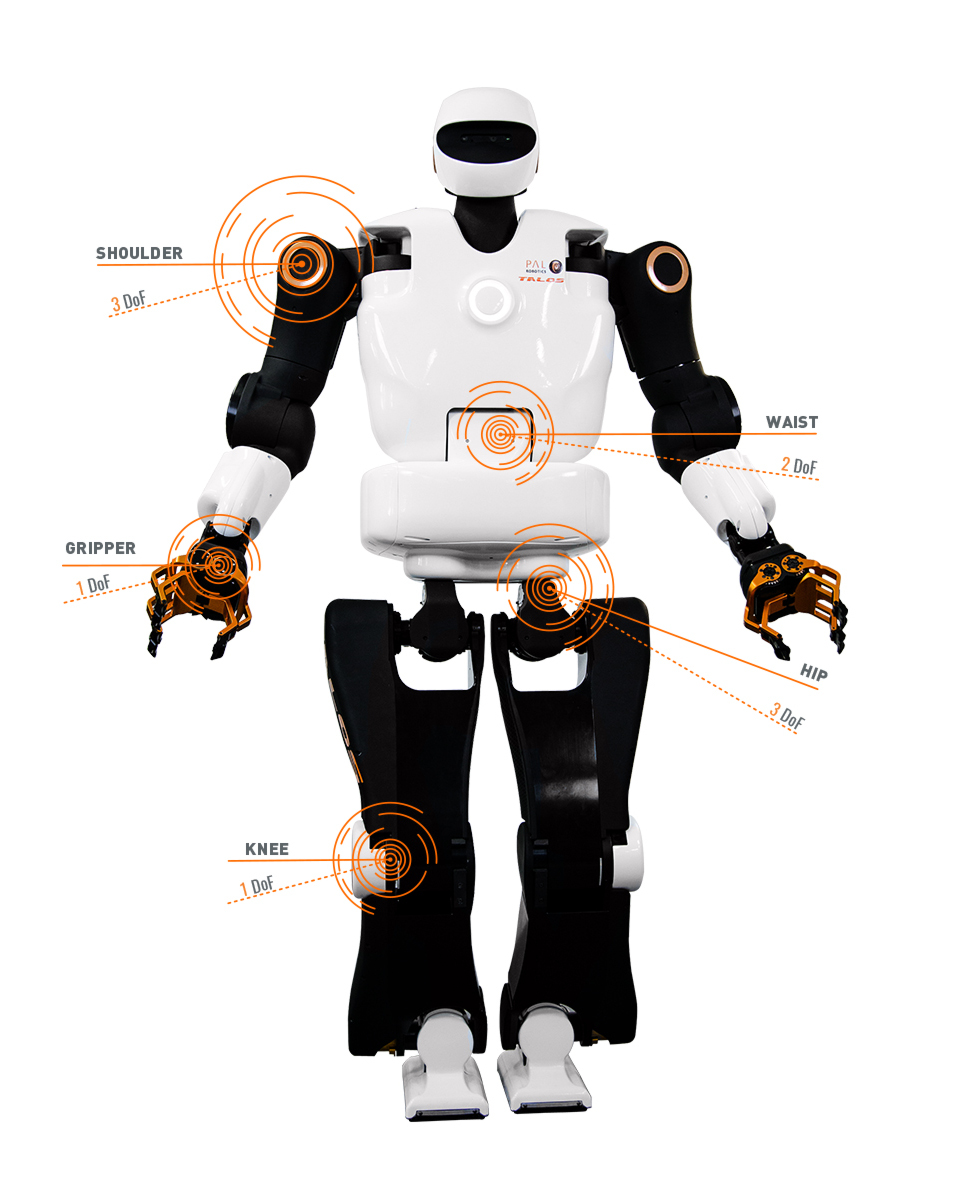
\includegraphics[width=0.6\textwidth]{chapter_introduction/figures/TALOS_FRONT.jpg}
    \caption[TALOS humanoid robot]{TALOS humanoid robot. Image taken from~\href{https://pal-robotics.com/robots/talos/}{\texttt{https://pal-robotics.com/robots/talos/}}
    \label{fig:talos}}
\end{figure}

\section{The TALOS Humanoid Robot\label{sec:talos}}
TALOS is a state-of-the-art humanoid robot that integrates the latest cutting-edge robotics technology~\citep{Stasse2017TALOS:Applications} designed and developed by PAL-Robotics -- Figure~\ref{fig:talos}.
By construction, the robot is capable of interacting with a human environment and targeting industrial applications. 
Since its release, several versions of TALOS have been produced, the following is the detailed description of \emph{Pyr\`{e}ne}, the first robot in the TALOS series built by PAL-Robotics, currently available and maintained by the Gepetto group at LAAS-CNRS in Toulouse. The content of this section is inspired by the official presentation of the robot available in \cite{Stasse2017TALOS:Applications}.
\begin{figure}[tpb]
\centering
    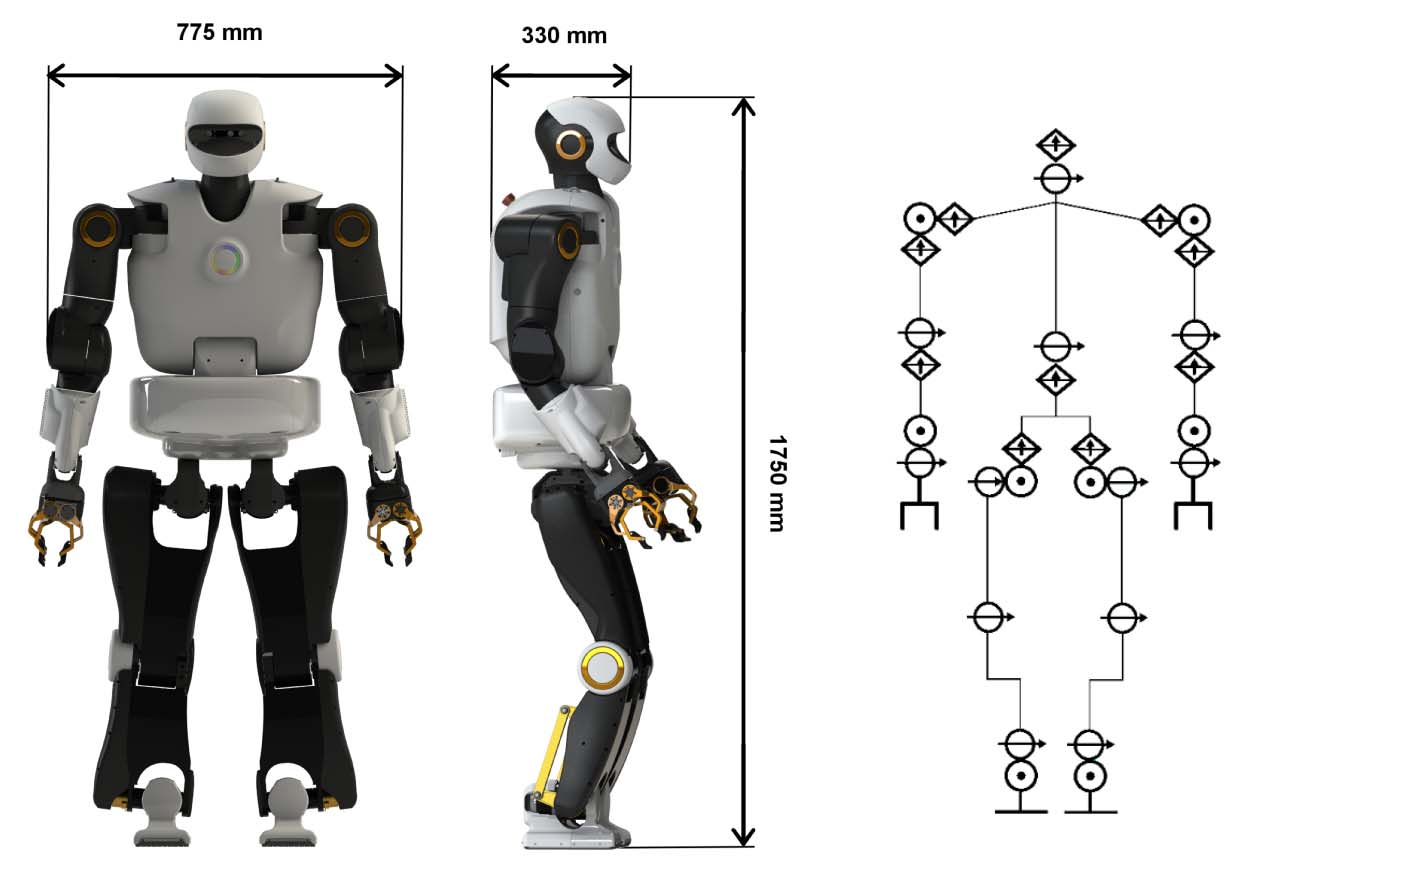
\includegraphics[width=\textwidth]{chapter_introduction/figures/talos_kinematics.png}
    \caption[Kinematics of Pyr\`{e}ne robot]{Kinematics of Pyr\`{e}ne robot. Image taken from~\citep{Stasse2017TALOS:Applications}    \label{fig:talos_kinematics}}
\end{figure}
\begin{figure}[tpb]
\centering
    \includegraphics{chapter_introduction/figures/talos_actuator.tikz}
    \caption{Structure of TALOS actuator \label{fig:talos_actuator}}
\end{figure}
\par
Figure~\ref{fig:talos_kinematics} presents the kinematics of Pyr\`{e}ne, which weights $\SI{95}{\kilo \gram}$ and is $\SI{1.75}{\meter}$ tall. It has $32$ actuated degrees of freedom in total and they are distributed as follows: $2$ joints in the head, $7$ joints in the arm, $3$ of which in the shoulder, $2$ in the elbow, and $2$ in the wrist, and $1$ joint in the gripper. $2$ joints allow controlling the pitch and yaw torso motion. Each leg has $6$ joints.
\par
Pyr\`{e}ne is equipped with Cobalt-Nickel-Manganese (Li-CNM) batteries that are capable of providing $\SI{75}{\volt}$ with a capacity of $\SI{15}{\ampere \hour}$. In the case a more power-consuming motion needs to be performed, the batteries can deliver current peaks of $\SI{150}{\ampere}$.
\par
Figure~\ref{fig:talos_actuator} presents the actuator structure of the TALOS robot. Each brushless DC motor is connected to a harmonic drive, which is attached to a torque sensor. The torque sensor is connected to a link.
Unlike iCub, each joint motor assembly is equipped with a torque sensor that can directly measure the torque applied on the load side. Furthermore, two high-precision encoders (19 bits each) measure the motor and joint positions.
Pyr\`{e}ne mounts an IMU at the level of its waist. This is involved in the estimation of the robot's base position and orientation. Similar to iCub, Pyr\`{e}ne is equipped with 6-axis force/torque sensors at the level of the hands and the feet. These sensors are often exploited to measure the contact force that the robot acts on the surrounding environment. 

\par
The robot comes with two processors, each with a dual i7 CPU running at 2.8 GHz. Each CPU contains two cores and is hyperthreaded, giving the machine a total of eight cores. 
The communication between the motors and sensors boards and the computers is implemented with an EtherCAT network~\citep{IEC61158-12019IndustrialSeries}. Because of TALOS' EtherCAT communication network, control loops can run at 2 kHz and up to 5 kHz, allowing for extremely reactive and dynamic motions.
\par
Pyr\`{e}ne runs Ubuntu 18.04 LTS as its operating system.
The ROS control system was used to develop the robot's low-level system.
The multimedia system uses stacks to provide navigation and map building. Furthermore, a complete Gazebo~\citep{Koenig04} simulation environment is provided.